%% ============================================================
%%  STANDARD PREAMBLE (article, lecture notes) -- exercise sheet,
%%  compiled separately from main.tex into exercise.pdf
%% ============================================================

% ---------- Document class and page layout ----------
\documentclass[11pt]{article}      % Basic document type, 11pt body text
\usepackage[margin=1in]{geometry}  % Sets page margins to 1 inch on all sides

% ---------- Paragraph style ----------
\usepackage{setspace}              % Lets you set the line spacing of the whole document
\setstretch{1.2}                   % Line spacing factor: 1.0 = single (default), 1.2 = slightly airy, 1.5 = very loose
\setlength{\parindent}{2em}        % First-line indent of each paragraph
\setlength{\parskip}{1\baselineskip} % Extra vertical gap between paragraphs
\setlength{\emergencystretch}{3em}  % Extra stretch so long inline math breaks without overfull lines

% ---------- Math ----------
\usepackage{amsmath,amssymb}       % Core math: align, cases, \text{}, \boxed{}, plus extra symbols (\mathbb, \hbar, ...)

% ---------- Figures ----------
\usepackage{graphicx}              % \includegraphics for the pre-built figures in figures/
\usepackage{float}                 % [H] keeps each figure at its place in the text
\usepackage{needspace}             % keeps a problem and its figure on one page

% ---------- Colors and boxes ----------
\usepackage{xcolor}                % Lets you use colors (\textcolor{red}{...})

% ---------- Text layout ----------
\usepackage{indentfirst}           % Indents the first paragraph after a heading (article class skips it by default)

% ---------- Hyperlinks (load last) ----------
\usepackage[hidelinks]{hyperref}   % Clickable TOC, \ref, \eqref, \cite; hidelinks = no colored text or boxes

% ---------- Equation numbering ----------
\numberwithin{equation}{section}   % Equation counter resets in each section
\renewcommand{\theequation}{\thesection.\arabic{equation}} % Displays numbers as section.equation, e.g. (2.3)

% ---------- Title block ----------
\title{Statistical Mechanics: Exercises}
\author{Duy M. Dao}
\date{\today}                      % Compile date; replace with a fixed date if you prefer

\begin{document}
\maketitle                         % Prints title, author, date

% Lettered parts (a), (b), ... for the exercises in this file.
\newenvironment{parts}
  {\begin{enumerate}\renewcommand{\theenumi}{\alph{enumi}}\renewcommand{\labelenumi}{(\theenumi)}}
  {\end{enumerate}}

\paragraph{Scope of the exercises.}
The exercises are selected from three problem collections:
A.~A.~Schekochihin and J.~Devriendt, \textit{Oxford Problem Sets 5--8: Statistical Mechanics} (2017), cited as [S];
D.~Cohen, \textit{Exercises in Statistical Mechanics} (Ben-Gurion University, 2019), cited as [C];
and D.~A.~R.~Dalvit, J.~Frastai and I.~D.~Lawrie, \textit{Problems on Statistical Mechanics} (IOP, 1999), cited as [D].
Only problems that the note covers and that require more than a substitution into one formula are included.
The problems are rewritten in the notation of the note, and some are merged or extended.
Problems on quantum gases, kinetic theory, interacting lattice models and continuous transitions are left out, because the note does not cover them yet.
The collections contain no problems on binary phase diagrams, so Section~11 of the note has no exercises here.
Each exercise names the related sections of the note and the source, and ends with an answer for checking.
Section~7 adds the five problems of Quiz~1 of the phase-diagram course, which cover Section~11 of the note and one ternary system. Full solutions with figures are in the separate file \texttt{quiz1.pdf}.
Guided exercises on point defects, built from the equations of a review article, are in the separate sheet \texttt{Freysoldt/freysoldt.pdf}.

\paragraph{Units and notation.}
\textcolor{red}{The Boltzmann constant $k_B$ is kept explicit, and $\beta = 1/(k_BT)$.
Where a problem needs the classical ideal gas, the canonical partition function of $N$ identical particles of mass $m$ in the volume $V$ is given as $Z_N = V^N/(N!\,\lambda_{\text{th}}^{3N})$, with the thermal wavelength $\lambda_{\text{th}} = h/\sqrt{2\pi m k_BT}$.}

% ============================================================
\section{Entropy Maximization}
% ============================================================

\paragraph{Exercise 1: Loaded die.}
A die has the outcomes $i = 1, \dots, 6$ with unknown probabilities $p_i$.
\begin{parts}
    \item With no information beyond normalization, find the MaxEnt distribution and the expected outcome $\langle i\rangle$.
    \item Many throws give the average $\bar\imath = 3.667$. Use MaxEnt with the constraint $\langle i\rangle = \bar\imath$ to show that $p_i = x^i/\sum_{j=1}^6 x^j$, with $x = e^{-\lambda}$ for the multiplier $\lambda$, and that $x$ solves
    \begin{equation*}
        \sum_{i=1}^6 (i - \bar\imath)\,x^i = 0.
    \end{equation*}
    \item Solve for $x$ numerically, list the $p_i$, and compare the entropy with $\ln 6$.
\end{parts}
\textit{Answer.} (a) $p_i = 1/6$ and $\langle i\rangle = 3.5$. (c) $x = 1.059$ ($\lambda = -0.057$), and $p_1, \dots, p_6 = 0.144$, $0.152$, $0.161$, $0.171$, $0.181$, $0.192$. The entropy is $1.787$, only $0.005$ below $\ln 6 = 1.792$, because the constraint is weak.\\
\textit{Related:} Sections~1.2 and~3 of the note. \textit{Source:} [S]~5.3.

\paragraph{Exercise 2: Additivity forces the logarithm.}
Suppose that the entropy of an isolated system is some function $S = \phi(\Omega)$ of the number of accessible microstates, with $\phi$ increasing.
\begin{parts}
    \item Two independent systems have $\Omega_1$ and $\Omega_2$ microstates. Show that additivity of the entropy requires $\phi(\Omega_1\Omega_2) = \phi(\Omega_1) + \phi(\Omega_2)$, and hence $\phi(1) = 0$ and $\phi(\Omega^n) = n\,\phi(\Omega)$ for every positive integer $n$.
    \item For integers $\Omega, M \ge 2$ and a large integer $n$, choose the integer $m$ with $M^m \le \Omega^n < M^{m+1}$. Use the monotonicity of $\phi$ to show that
    \begin{equation*}
        \left|\frac{\phi(\Omega)}{\phi(M)} - \frac{\ln\Omega}{\ln M}\right| \le \frac{1}{n},
    \end{equation*}
    and conclude that $\phi(\Omega) = k\ln\Omega$ with a constant $k > 0$.
    \item Show that the Gibbs--Shannon entropy of a uniform distribution over $\Omega$ microstates has this form, and explain why the note sets $k = k_B$.
\end{parts}
\textit{Answer.} (b) Both $\phi(\Omega)/\phi(M)$ and $\ln\Omega/\ln M$ lie in $[m/n, (m+1)/n)$. The ratio $k = \phi(M)/\ln M$ is therefore the same for every $M$. (c) $S = \ln\Omega$ for $p_i = 1/\Omega$, and $k_B$ only fixes the units.\\
\textit{Related:} Sections~1.1 and~2 of the note. \textit{Source:} [C]~1043.

% ============================================================
\section{The Microcanonical Ensemble}
% ============================================================

\paragraph{Exercise 3: Two-level system and negative temperature.}
$N$ distinguishable, non-interacting particles each have the energy $-\varepsilon$ or $+\varepsilon$. The system is isolated with the energy $E$, so that $n = (N + E/\varepsilon)/2$ particles occupy the upper level.
\begin{parts}
    \item Find $S(E)$ for $N, n \gg 1$, and sketch $S$ against $E$.
    \item From $1/T = \partial S/\partial E$, find $T(E)$. Show that $T < 0$ for $E > 0$, and explain why such states are hotter than any state with $T > 0$.
    \item The system at $T < 0$ touches a heat bath at $T_0 > 0$. Use the entropy change $\delta S = k_B(\beta_1 - \beta_2)\,\delta U_1$ of Section~3.4 of the note to find the direction of the energy flow.
    \item Find the entropy change from $T = 0^+$ to $T \to \pm\infty$ and express it in bits.
    \item Explain why an ideal gas in a box cannot reach $T < 0$.
\end{parts}
\textit{Answer.} (a) $S = -Nk_B[x\ln x + (1 - x)\ln(1 - x)]$ with $x = n/N$, maximal at $E = 0$. (b) $\beta = (2\varepsilon)^{-1}\ln[(N - n)/n] = -(2\varepsilon)^{-1}\ln[(N\varepsilon + E)/(N\varepsilon - E)]$. As $E$ increases, $\beta$ decreases continuously from $+\infty$ through $0$ to $-\infty$. (c) Energy flows from the system to the bath, because the bath has the larger $\beta$. (d) $\Delta S = Nk_B\ln 2$, that is, $N$ bits. (e) The kinetic energy has no upper bound, so $S(E)$ increases for all $E$.\\
\textit{Related:} Sections~2 and~3.4 of the note. \textit{Source:} [C]~1047; [D]~3.6.

\paragraph{Exercise 4: Frenkel defects.}
A crystal has $N$ atoms on $N$ lattice sites and $M$ interstitial sites, with $M$ of order $N$. Moving an atom from a lattice site to an interstitial site costs the energy $\omega$. Let $x = e^{-\beta\omega}$.
\begin{parts}
    \item Show that the canonical partition function is
    \begin{equation*}
        Z(x) = \sum_{n} \binom{N}{n}\binom{M}{n}\,x^n.
    \end{equation*}
    \item Treat $n$ as continuous, with $d\ln n!/dn \approx \ln n$, and find the largest term. Show that $n^2/[(N - n)(M - n)] = x$, and hence $\bar n \approx \sqrt{NM}\,e^{-\beta\omega/2}$ for $x \ll 1$.
    \item Interpret the condition of part~(b) as a law of mass action for the reaction ``lattice atom $\rightleftharpoons$ vacancy $+$ interstitial''.
    \item Keep only the largest term in $\ln Z$ and find $F$, $U$, $S$ and $C_V$ for $x \ll 1$.
    \item Explain why a Gaussian sum around the largest term changes $\ln Z$ only by $O(\ln\bar n)$.
\end{parts}
\textit{Answer.} (b) For $N = M = 4000$ and $x = e^{-12}$, the exact mean is $9.64$ and the approximation gives $9.92$. (d) $\ln Z \approx 2\bar n$, so $F = -2k_BT\bar n$, $U = \bar n\omega$, $S = k_B\bar n(2 + \beta\omega)$ and $C_V = 2k_B\bar n(\beta\omega/2)^2$. The factor $1/2$ in the exponent of $\bar n$ reflects that each defect creates two independent objects, a vacancy and an interstitial.\\
\textit{Related:} Sections~2, 3 and~3.3 of the note. \textit{Source:} [C]~2311.

% ============================================================
\section{The Canonical Ensemble}
% ============================================================

\paragraph{Exercise 5: Elastic chain and superfluous constraints.}
\textcolor{red}{Here, $\tau$ denotes a tension and $\Lambda$ the length of a chain.}
A one-dimensional chain has $N$ segments. Each segment is horizontal, with the length $a$ and the energy $0$, or vertical, with the length $0$ and the energy $\tau a$, where $\tau$ is a fixed tension.
\begin{parts}
    \item Find the canonical partition function and the mean energy $U(T)$.
    \item Show that the mean length is $\langle\Lambda\rangle = Na - U/\tau$. For $\beta\tau a \ll 1$, show that $\tau = A k_BT(\langle\Lambda\rangle - \Lambda_0)$, a Hooke law, and find $A$ and $\Lambda_0$. Explain why a hotter chain needs a larger tension for the same length.
    \item Find the heat capacity at fixed $\tau$, and explain why it vanishes at low and at high temperature.
    \item Find the condition on $U$ for $T < 0$.
    \item Maximize the entropy with two constraints, $\langle E\rangle = U$ and $\langle\Lambda\rangle = \Lambda$, with the multipliers $\beta$ and $\sigma$. Show that a solution exists only if $\Lambda = Na - U/\tau$, and that only the combination $\beta - \sigma/\tau$ is determined. Relate this result to the uniqueness condition for the multipliers in Section~5 of the note.
\end{parts}
\textit{Answer.} (a) $Z = (1 + e^{-\beta\tau a})^N$ and $U = N\tau a/(e^{\beta\tau a} + 1)$. (b) $\Lambda_0 = Na/2$ and $A = 4/(Na^2)$. The tension opposes the entropy, which favors the disordered half-and-half state, and the entropic restoring force grows with $T$. (c) $C = Nk_B(\beta\tau a)^2 e^{\beta\tau a}/(e^{\beta\tau a} + 1)^2$, the Schottky form, with a maximum near $k_BT \approx 0.42\,\tau a$. (d) $U > N\tau a/2$. (e) Every microstate satisfies $E + \tau\Lambda = N\tau a$, so the covariance matrix of $(E, \Lambda)$ is singular.\\
\textit{Related:} Sections~1.2, 3 and~5 of the note. \textit{Source:} [S]~5.5.

\paragraph{Exercise 6: Zipper model and the thermodynamic limit.}
A double-stranded molecule has $N$ links that open only in sequence from one end, and the last link never opens. An open link costs the energy $\varepsilon$ and has $g$ orientations. A state with $p$ open links has the energy $p\varepsilon$ and the degeneracy $g^p$.
\begin{parts}
    \item With $x = g\,e^{-\beta\varepsilon}$, show that $Z = (1 - x^N)/(1 - x)$.
    \item Find $\langle p\rangle$, and show that $\langle p\rangle/N \to 0$ for $x < 1$ and $\langle p\rangle/N \to 1$ for $x > 1$ as $N \to \infty$.
    \item Show that $\langle p\rangle \approx (N - 1)/2 + (x - 1)(N^2 - 1)/12$ near $x = 1$, and find the transition temperature $T_c$.
    \item Find the heat capacity at $x = 1$ and show that it grows as $N^2$.
    \item Explain why the free energy is analytic in $T$ for every finite $N$, and why a transition nevertheless appears in the limit. Which order is the transition?
\end{parts}
\textit{Answer.} (b) $\langle p\rangle = x/(1 - x) - Nx^N/(1 - x^N)$. For $N = 500$, $\langle p\rangle/N = 0.04$, $0.50$ and $0.96$ at $x = 0.95$, $1$ and $1.05$. (c) $T_c = \varepsilon/(k_B\ln g)$. The slope is the variance $(N^2 - 1)/12$ of a uniform distribution. (d) $C = k_B(\ln g)^2(N^2 - 1)/12$. (e) $Z$ is a polynomial in $x$, so $\ln Z$ is analytic for finite $N$. In the limit, the fraction of open links jumps from $0$ to $1$ with the latent heat $\varepsilon$ per link, a first-order transition.\\
\textit{Related:} Sections~3 and~10 of the note. \textit{Source:} [C]~2360.

\paragraph{Exercise 7: Free energy of a perturbed Hamiltonian.}
A classical system has the Hamiltonian $\mathcal{H} = \mathcal{H}_0 + \lambda\mathcal{H}_1$. Let $F_0$ and $\langle\cdot\rangle_0$ denote the free energy and the averages at $\lambda = 0$.
\begin{parts}
    \item Show that $e^{-\beta(F - F_0)} = \langle e^{-\beta\lambda\mathcal{H}_1}\rangle_0$.
    \item Expand in $\lambda$ and show that
    \begin{equation*}
        F = F_0 + \lambda\langle\mathcal{H}_1\rangle_0 - \frac{\beta\lambda^2}{2}\,\mathrm{Var}_0(\mathcal{H}_1) + \frac{\beta^2\lambda^3}{6}\,\kappa_3 + O(\lambda^4),
    \end{equation*}
    where $\kappa_3 = \langle(\mathcal{H}_1 - \langle\mathcal{H}_1\rangle_0)^3\rangle_0$.
    \item Show that $\partial^2F/\partial\lambda^2 = -\beta\,\mathrm{Var}_\lambda(\mathcal{H}_1) \le 0$ for every $\lambda$, and deduce the Gibbs--Bogoliubov bound $F \le F_0 + \lambda\langle\mathcal{H}_1\rangle_0$.
    \item Find $U = \langle\mathcal{H}\rangle$ to first order in $\lambda$.
\end{parts}
\textit{Answer.} (b) The expansion is the cumulant expansion of $\ln\langle e^{-\beta\lambda\mathcal{H}_1}\rangle_0$. (c) $F(\lambda)$ is concave, so the curve lies below the tangent at $\lambda = 0$. (d) $U = U_0 + \lambda\left[\langle\mathcal{H}_1\rangle_0 - \beta\,\mathrm{Cov}_0(\mathcal{H}_0, \mathcal{H}_1)\right] + O(\lambda^2)$.\\
\textit{Related:} Sections~3 and~3.3 of the note. \textit{Source:} [D]~3.13.

% ============================================================
\section{Thermodynamic Potentials and Legendre Transformations}
% ============================================================

\paragraph{Exercise 8: Heat capacities and compressibilities.}
\textcolor{red}{Here, $\alpha_P = V^{-1}(\partial V/\partial T)_P$ is the thermal expansivity, $\kappa_T = -V^{-1}(\partial V/\partial P)_T$ the isothermal compressibility and $\kappa_S = -V^{-1}(\partial V/\partial P)_S$ the adiabatic compressibility, all at fixed $N$.}
\begin{parts}
    \item From the equality of the mixed second derivatives of $F(T, V, N)$ and of $G(T, P, N)$, derive the Maxwell relations $(\partial S/\partial V)_T = (\partial P/\partial T)_V$ and $(\partial S/\partial P)_T = -(\partial V/\partial T)_P$.
    \item Show that $T\,dS = C_V\,dT + T(\alpha_P/\kappa_T)\,dV$ and $T\,dS = C_P\,dT - TV\alpha_P\,dP$.
    \item Prove that
    \begin{equation*}
        C_P - C_V = \frac{TV\alpha_P^2}{\kappa_T},
        \qquad
        \frac{C_P}{C_V} = \frac{\kappa_T}{\kappa_S}.
    \end{equation*}
    \item Express $C_P$ and $C_V$ in terms of $T$, $V$, $\alpha_P$, $\kappa_T$ and $\kappa_S$.
    \item Use the stability conditions of the note to show that $C_P \ge C_V > 0$ and $\kappa_T \ge \kappa_S > 0$.
\end{parts}
\textit{Answer.} (b) $(\partial P/\partial T)_V = \alpha_P/\kappa_T$ by the cyclic rule. (d) $C_P = TV\alpha_P^2/(\kappa_T - \kappa_S)$ and $C_V = TV\alpha_P^2\kappa_S/[\kappa_T(\kappa_T - \kappa_S)]$. (e) $C_V > 0$ and $\kappa_T > 0$ follow from the concavity of $S$ and the convexity of $F$ in $V$. Then $C_P - C_V \ge 0$, and $\kappa_S = \kappa_TC_V/C_P$.\\
\textit{Related:} Sections~3.3, 4.4 and~5.3 of the note. \textit{Source:} [D]~2.4.

\paragraph{Exercise 9: Rubber band in the constant-tension ensemble.}
A polymer has $N$ monomers on a line. Each monomer has the length $a$ and the energy $E_a$, or the length $b$ and the energy $E_b$, with $a > b$. The polymer is held at the temperature $T$ under the tension $\tau$.
\begin{parts}
    \item Maximize the entropy with the constraints $\langle E\rangle$ and $\langle\Lambda\rangle$, identify the multiplier of the length as $-\beta\tau$, and show that
    \begin{equation*}
        \Gamma(T, \tau) = \left[e^{-\beta(E_a - \tau a)} + e^{-\beta(E_b - \tau b)}\right]^N.
    \end{equation*}
    \item Show that $G(N, \tau, T) = -k_BT\ln\Gamma = F - \tau\Lambda$ is the Legendre transform of $F(N, \Lambda, T)$ in $\Lambda$. Name the ensemble by the natural variables of $G$, and find $\Lambda = -\partial G/\partial\tau$.
    \item Find $\Lambda(T \to \infty, \tau)$. For $E_a = E_b$ and weak tension, show that $\tau = 4k_BT(\Lambda - \Lambda_\infty)/[N(a - b)^2]$.
    \item At $\tau = 0$ and $E_a = E_b$, find the distribution $P(\Lambda)$ of the length for large $N$. Show that the entropic force $\tau = -k_BT\,\partial\ln P/\partial\Lambda$ reproduces part~(c).
    \item Let each monomer take any length in $[b, a]$ with equal energy. Find $\Gamma$ and $\Lambda(T, \tau)$.
\end{parts}
\textit{Answer.} (b) The $N\tau T$ ensemble, with $\Lambda = N\left[b + (a - b)\,p_a\right]$ and $p_a = \{1 + e^{\beta[(E_a - \tau a) - (E_b - \tau b)]}\}^{-1}$. (c) $\Lambda_\infty = N(a + b)/2$. (d) $P(\Lambda)$ is Gaussian with the mean $\Lambda_\infty$ and the variance $N(a - b)^2/4$. (e) $\Gamma = \left[(e^{\beta\tau a} - e^{\beta\tau b})/(\beta\tau(a - b))\right]^N$ and $\Lambda = N\left[(a e^{\beta\tau a} - b e^{\beta\tau b})/(e^{\beta\tau a} - e^{\beta\tau b}) - k_BT/\tau\right]$.\\
\textit{Related:} Sections~1.2, 4.4 and~4.5 of the note. \textit{Source:} [C]~2351.

% ============================================================
\section{The Grand Canonical Ensemble}
% ============================================================

\paragraph{Exercise 10: The grand canonical distribution from a reservoir.}
A small system exchanges energy and particles with a large reservoir, and the two together are isolated, with the total energy $E_{\text{tot}}$ and the total particle number $N_{\text{tot}}$.
\begin{parts}
    \item Assume equal probabilities for the microstates of the isolated whole. Show that the probability of a system microstate $i$ is proportional to $\Omega_R(E_{\text{tot}} - E_i, N_{\text{tot}} - N_i)$.
    \item Expand $S_R = k_B\ln\Omega_R$ to first order and recover $p_i \propto e^{-\beta(E_i - \mu N_i)}$. Identify $T$ and $\mu$ with derivatives of $S_R$.
    \item Estimate the second-order terms and show that they vanish as the reservoir becomes infinitely large.
    \item Compare this derivation with the MaxEnt derivation in Section~5 of the note. Which assumption replaces the constraints on $\langle E\rangle$ and $\langle N\rangle$?
\end{parts}
\textit{Answer.} (b) $1/T = \partial S_R/\partial E$ and $-\mu/T = \partial S_R/\partial N$. (c) The second derivatives scale as $1/N_R$, so their terms are of order $E_i^2/N_R$. (d) The reservoir fixes $T$ and $\mu$ through the reservoir entropy, whereas MaxEnt fixes the multipliers through the measured averages. Both give the same distribution.\\
\textit{Related:} Sections~3.4 and~5 of the note. \textit{Source:} [S]~6.11.

\paragraph{Exercise 11: Energy fluctuations with particle exchange.}
\textcolor{red}{Here, $z = e^{\beta\mu}$ denotes the fugacity.}
\begin{parts}
    \item From $\ln\Xi(\beta, z)$ at fixed $V$, show that $\mathrm{Var}_G(E) = -(\partial U/\partial\beta)_z$, $\mathrm{Var}(N) = z(\partial N/\partial z)_\beta$, and $\mathrm{Cov}(E, N) = z(\partial U/\partial z)_\beta = -(\partial N/\partial\beta)_z$.
    \item In the thermodynamic limit, $U$ in the grand canonical ensemble equals $U(\beta, V, N)$ in the canonical ensemble with $N = N(\beta, z)$. Use the chain rule to prove
    \begin{equation*}
        \mathrm{Var}_G(E) = \mathrm{Var}_C(E) + \left(\frac{\partial U}{\partial N}\right)_{T,V}^2\mathrm{Var}(N).
    \end{equation*}
    \item Explain why the grand canonical energy fluctuation exceeds the canonical one.
    \item For the monatomic ideal gas, with $U = \tfrac32Nk_BT$ and $\mathrm{Var}(N) = N$, find the ratio $\mathrm{Var}_G(E)/\mathrm{Var}_C(E)$.
\end{parts}
\textit{Answer.} (b) $(\partial U/\partial\beta)_z = (\partial U/\partial\beta)_N + (\partial U/\partial N)_\beta(\partial N/\partial\beta)_z$, and $-(\partial N/\partial\beta)_z = (\partial U/\partial N)_\beta\,\mathrm{Var}(N)$. (c) The exchanged particles carry energy. (d) $\mathrm{Var}_G(E) = \tfrac{15}{4}N(k_BT)^2$ and $\mathrm{Var}_C(E) = \tfrac32N(k_BT)^2$, so the ratio is $5/2$.\\
\textit{Related:} Sections~3.3, 5 and~5.1 of the note. \textit{Source:} [D]~3.28.

\paragraph{Exercise 12: Particle-number fluctuations and compressibility.}
\begin{parts}
    \item Use the Gibbs--Duhem relation at fixed $T$, $dP = (N/V)\,d\mu$, to show that $(\partial N/\partial\mu)_{T,V} = N^2\kappa_T/V$. Hence express $\mathrm{Var}(N)/N$ through $\kappa_T$.
    \item Show that the third cumulant is $\langle(N - \langle N\rangle)^3\rangle = (k_BT)^2(\partial^2N/\partial\mu^2)_{T,V}$.
    \item For the classical ideal gas, show that $\Xi = \exp(zV/\lambda_{\text{th}}^3)$, that all cumulants of $N$ equal $\langle N\rangle$, and that $N$ has the Poisson distribution $P(N) = \langle N\rangle^Ne^{-\langle N\rangle}/N!$.
    \item Explain why $\mathrm{Var}(N)/N$ grows without bound as a fluid approaches the critical point.
\end{parts}
\textit{Answer.} (a) $\mathrm{Var}(N)/N = k_BT\,(N/V)\,\kappa_T$. (b) The $n$th cumulant is $(k_BT)^{n-1}\partial^{n-1}N/\partial\mu^{n-1}$. (c) $N = zV/\lambda_{\text{th}}^3 \propto e^{\beta\mu}$, so every derivative $k_BT\,\partial/\partial\mu$ returns $N$. (d) $\kappa_T \to \infty$ at the critical point, where $\partial P/\partial v = 0$.\\
\textit{Related:} Sections~5.1 and~5.7 of the note. \textit{Source:} [D]~2.5; [C]~1027; [S]~6.9.

\paragraph{Exercise 13: Langmuir adsorption.}
A classical ideal gas at the pressure $P$ and the temperature $T$ is in contact with a wall that has $N_0$ independent sites. Each site is empty, with the energy $0$, or holds one molecule, with the energy $-\varepsilon$.
\begin{parts}
    \item Use the result of Exercise~12 to show that the fugacity of the gas is $z = P\lambda_{\text{th}}^3/(k_BT)$.
    \item Treat the sites as a grand canonical system with the same $T$ and $\mu$ as the gas. Find the grand partition function of one site and the mean number of adsorbed molecules $\langle N_s\rangle$.
    \item Write the coverage $\theta = \langle N_s\rangle/N_0$ as $P/(P + P_0(T))$ and find $P_0(T)$. Discuss the limits of low and high pressure.
    \item Find $\mathrm{Var}(N_s)$, and explain why it vanishes at full coverage.
\end{parts}
\textit{Answer.} (b) $\xi = 1 + z e^{\beta\varepsilon}$ and $\langle N_s\rangle = N_0 z e^{\beta\varepsilon}/(1 + z e^{\beta\varepsilon})$. (c) $P_0 = (k_BT/\lambda_{\text{th}}^3)\,e^{-\beta\varepsilon}$. At low pressure $\theta \approx P/P_0$ (Henry's law), and at high pressure $\theta \to 1$. (d) $\mathrm{Var}(N_s) = N_0\theta(1 - \theta)$.\\
\textit{Related:} Sections~5 and~5.5 of the note. \textit{Source:} [D]~3.25.

\paragraph{Exercise 14: The $NPT$ ensemble of an ideal gas.}
The partition function of the $NPT$ ensemble in the note is $\Gamma = \sum_i e^{-\beta(E_i + PV_i)}$. For a gas in a container of variable volume, replace the sum over volumes by $\int_0^\infty dV/\Delta V$, where $\Delta V$ is a ``quantum of volume''.
\begin{parts}
    \item With $Z_N(V)$ of the classical ideal gas, show that
    \begin{equation*}
        \Gamma = \frac{1}{\Delta V\,\lambda_{\text{th}}^{3N}}\left(\frac{k_BT}{P}\right)^{N+1}.
    \end{equation*}
    \item Find $G = -k_BT\ln\Gamma$. Show that $G = N\mu$ with $\mu = k_BT\ln(P\lambda_{\text{th}}^3/k_BT)$, up to a term that does not grow with $N$, and find the condition on $\Delta V$ for that term to be negligible.
    \item Find $\langle V\rangle = (\partial G/\partial P)_{T,N}$ and the equation of state.
    \item Find $\mathrm{Var}(V)/\langle V\rangle^2$, and relate it to $\kappa_T$.
\end{parts}
\textit{Answer.} (b) $G = Nk_BT\ln(P\lambda_{\text{th}}^3/k_BT) - k_BT\ln(k_BT/P\Delta V)$. The second term is negligible if $|\ln(\langle V\rangle/N\Delta V)| \ll N$, which holds for any physically reasonable $\Delta V$. (c) $\langle V\rangle = (N + 1)k_BT/P \approx Nk_BT/P$. (d) $\mathrm{Var}(V) = k_BT\langle V\rangle\kappa_T$, so $\mathrm{Var}(V)/\langle V\rangle^2 = 1/(N + 1)$.\\
\textit{Related:} Sections~5.3 and~5.4 of the note. \textit{Source:} [S]~6.12.

\paragraph{Exercise 15: Mixing gases at different temperatures.}
The monatomic classical ideal gas has the entropy
\begin{equation*}
    S(U, V, N) = Nk_B\left[\ln\!\left(\frac{V}{N}\left(\frac{4\pi mU}{3Nh^2}\right)^{3/2}\right) + \frac52\right].
\end{equation*}
Two such gases, with equal particle masses, occupy the volumes $V_1$ and $V_2$, with the particle numbers $N_1$ and $N_2$ and the temperatures $T_1$ and $T_2$. The wall between them is removed, and the combined system comes to equilibrium in $V = V_1 + V_2$.
\begin{parts}
    \item Find the final temperature.
    \item Find $\Delta S$ when the two gases are identical and when they are different species.
    \item Show that the difference between the two results is
    \begin{equation*}
        \Delta S_{\text{diff}} - \Delta S_{\text{ident}} = -Nk_B\left[x_1\ln x_1 + x_2\ln x_2\right],
        \qquad x_i = N_i/N,
    \end{equation*}
    independent of $T_1$, $T_2$, $V_1$ and $V_2$.
    \item Relate the result of part~(c) to $\Delta S_{\text{mix}} \ge 0$ in Section~5.6 of the note and to the ideal-solution model of Section~11.7.
\end{parts}
\textit{Answer.} (a) $T_f = (N_1T_1 + N_2T_2)/N$. (b)
\begin{equation*}
    \Delta S_{\text{ident}} = \tfrac32k_B\left[N\ln T_f - N_1\ln T_1 - N_2\ln T_2\right] + k_B\left[N\ln\frac{V}{N} - N_1\ln\frac{V_1}{N_1} - N_2\ln\frac{V_2}{N_2}\right],
\end{equation*}
and $\Delta S_{\text{diff}}$ has $k_B[N_1\ln(V/V_1) + N_2\ln(V/V_2)]$ as the second bracket. (d) The difference is the ideal mixing entropy, which the ideal-solution model assumes for the composition dependence of $g$.\\
\textit{Related:} Sections~5.6 and~11.7 of the note. \textit{Source:} [C]~1045; [S]~5.6.

% ============================================================
\section{First-Order Phase Transitions and the Unary System}
% ============================================================

\paragraph{Exercise 16: Critical point of a model fluid.}
\begin{parts}
    \item Below $T_c$, a model isotherm $P(v)$ has a region with $\partial P/\partial v > 0$. Use the convexity of $f(v)$ in Section~10.3 of the note to explain why this region is unstable. Show that the region shrinks to one point at $T_c$, so that the critical point satisfies
    \begin{equation*}
        \left(\frac{\partial P}{\partial v}\right)_T = 0,
        \qquad
        \left(\frac{\partial^2P}{\partial v^2}\right)_T = 0.
    \end{equation*}
    \item The Dieterici equation of state per particle is $P(v - b) = k_BT\,e^{-a/(k_BTv)}$. Find $T_c$, $v_c$ and $P_c$.
    \item In the reduced variables $\tilde P = P/P_c$, $\tilde T = T/T_c$ and $\tilde v = v/v_c$, show that $\tilde P(2\tilde v - 1) = \tilde T\exp[2(1 - 1/\tilde T\tilde v)]$, a law of corresponding states.
    \item Compare the critical ratio $P_cv_c/k_BT_c$ with the van der Waals value $3/8$ and with the measured values of about $0.29$ for simple gases.
\end{parts}
\textit{Answer.} (a) $\partial P/\partial v = -\partial^2f/\partial v^2$, which must be $\le 0$. At $T_c$, the minimum and the maximum of $P(v)$ merge into an inflection point. (b) $T_c = a/(4k_Bb)$, $v_c = 2b$ and $P_c = a/(4e^2b^2)$. (d) $P_cv_c/k_BT_c = 2/e^2 = 0.271$.\\
\textit{Related:} Section~10.3 of the note. \textit{Source:} [S]~8.2.

\paragraph{Exercise 17: Van der Waals coexistence near the critical point.}
The reduced van der Waals equation of state is $\tilde P = 8\tilde T/(3\tilde v - 1) - 3/\tilde v^2$.
\begin{parts}
    \item Show that the critical isotherm satisfies $\tilde P - 1 \approx -\tfrac32(\tilde v - 1)^3$.
    \item On the critical isochore $\tilde v = 1$ above $T_c$, show that $P_c\kappa_T = [6(\tilde T - 1)]^{-1}$.
    \item Below $T_c$, apply Maxwell's equal-area rule from Section~10.3 of the note to show that $\tilde v_g - \tilde v_l \approx 4(1 - \tilde T)^{1/2}$.
    \item Use the Clapeyron equation to show that the latent heat per particle vanishes as $\ell \approx 6k_BT_c(1 - \tilde T)^{1/2}$.
\end{parts}
\textit{Answer.} (c) A numerical Maxwell construction gives $(\tilde v_g - \tilde v_l)/(1 - \tilde T)^{1/2} = 4.12$, $4.01$ and $4.001$ for $1 - \tilde T = 10^{-2}$, $10^{-3}$ and $10^{-4}$. (d) $d\tilde P/d\tilde T \to 4$ on the coexistence curve at $T_c$, and $P_cv_c = \tfrac38k_BT_c$. The latent heat and $\Delta v$ vanish together at $T_c$, as Section~10.3 of the note states.\\
\textit{Related:} Sections~10.2 and~10.3 of the note. \textit{Source:} [D]~5.8.

\paragraph{Exercise 18: Latent heat along the vaporization curve.}
A liquid is incompressible and does not expand with temperature. The vapor volume per particle $v_g$ is much larger than $v_l$.
\begin{parts}
    \item Differentiate $\ell = T(s_g - s_l)$ along the coexistence curve. Use a Maxwell relation and the Clapeyron equation to show that
    \begin{equation*}
        \frac{d\ell}{dT} = \frac{\ell}{T} + \Delta c_P - \frac{\ell}{v_g}\left(\frac{\partial v_g}{\partial T}\right)_P,
        \qquad \Delta c_P = c_{P,g} - c_{P,l}.
    \end{equation*}
    \item For an ideal-gas vapor and a constant $\Delta c_P$, show that $\ell = \ell_0 + \Delta c_P\,T$.
    \item A saturated vapor expands adiabatically. Show that some liquid condenses if
    \begin{equation*}
        c_{P,l} + T\,\frac{d}{dT}\!\left(\frac{\ell}{T}\right) < 0.
    \end{equation*}
    \item Check the condition for water at $100\,^\circ$C, with $c_{P,l} = 75.3$, $c_{P,g} = 33.6$~J~mol$^{-1}$~K$^{-1}$ and $\ell = 40.7$~kJ~mol$^{-1}$.
\end{parts}
\textit{Answer.} (a) $(\partial s/\partial P)_T = -(\partial v/\partial T)_P$ and $dP/dT = \ell/(Tv_g)$. (c) The entropy of the saturated vapor along the curve is $s_l + \ell/T$, with $ds_l/dT = c_{P,l}/T$. If this entropy decreases with $T$, an adiabat that starts on the curve enters the two-phase region on cooling. (d) The left side equals $-75$~J~mol$^{-1}$~K$^{-1}$, so expanding water vapor condenses, as in cloud formation.\\
\textit{Related:} Sections~4.5, 10.2 and~10.3 of the note. \textit{Source:} [S]~8.8.

\paragraph{Exercise 19: Boiling point and altitude.}
An isothermal atmosphere at $T_A = 300.15$~K consists of an ideal gas with the molar mass $30$~g~mol$^{-1}$, and the pressure at sea level is $P_0$. A liquid with the molar latent heat $1000$~cal~mol$^{-1}$ boils at $105\,^\circ$C at sea level and at $95\,^\circ$C on the top of a mountain.
\begin{parts}
    \item Use the Boltzmann distribution of a molecule in the gravitational potential $mgh$ to find $P_A(h)$.
    \item Integrate the Clausius--Clapeyron equation to find the vapor pressure of the liquid $P_{\text{vap}}(T)$, with $P_{\text{vap}}(378.15~\text{K}) = P_0$.
    \item Find the height of the mountain.
\end{parts}
\textit{Answer.} (a) $P_A = P_0\exp(-Mgh/RT_A)$. (b) $P_{\text{vap}} = P_0\exp[-(\ell_m/R)(1/T - 1/378.15~\text{K})]$, with the molar latent heat $\ell_m$. (c) $h = (\ell_mT_A/Mg)(1/368.15 - 1/378.15)~\text{K}^{-1} = 307$~m.\\
\textit{Related:} Sections~3 and~10.3 of the note. \textit{Source:} [C]~5955.

\paragraph{Exercise 20: Cooling by solidification in helium-3.}
Below about $1$~K, the entropy per particle of liquid $^3$He is $s_l = (\pi^2/2)k_BT/T_F$ with $T_F \approx 5$~K. In the solid, the nuclear spins $1/2$ are disordered and independent, so that $s_s = k_B\ln 2$. The solid is denser, and $\Delta v = v_l - v_s > 0$ is independent of $T$.
\begin{parts}
    \item Find the temperature $T^*$ at which the two phases have equal entropy.
    \item Use the Clapeyron equation to show that the melting curve is
    \begin{equation*}
        P(T) = P^* + \frac{\pi^2k_B}{4T_F\,\Delta v}\,(T - T^*)^2,
    \end{equation*}
    with a minimum at $T^*$. Explain why the liquid is the low-entropy phase below $T^*$.
    \item State the order of the transition and find the jump in the heat capacity per particle.
    \item The liquid at $T_0 < T^*$ is compressed adiabatically. Assume that $T_F$ does not depend on the pressure. Show that $T$ stays at $T_0$ until the melting curve is reached.
    \item Further compression converts liquid to solid at fixed total entropy. Show that the system moves down the melting curve to lower $T$, with the solid fraction $n_s(T) = (T_0 - T)/(T^* - T)$.
\end{parts}
\textit{Answer.} (a) $T^* = (2\ln 2/\pi^2)\,T_F = 0.70$~K for $T_F = 5$~K (measured: $0.32$~K). (b) $s_l - s_s = (\pi^2k_B/2T_F)(T - T^*)$. (c) First order, with $\Delta c = (\pi^2/2)k_BT/T_F$ and $c_s = 0$. (e) The solid has the larger entropy below $T^*$, so freezing at fixed $S$ absorbs heat from the liquid. This effect is Pomeranchuk cooling.\\
\textit{Related:} Sections~10.2 and~10.3 of the note. \textit{Source:} [C]~4552.

% ============================================================
\section{Binary and Ternary Phase Diagrams}
% ============================================================

\paragraph{Exercise 21: Compound with a eutectic side and a peritectic side.}
The system $A$--$B$ forms the congruently melting compound $A_xB_y$, denoted $\gamma$. Alloys between $A$ and $A_xB_y$ are of the eutectic type, and alloys between $A_xB_y$ and $B$ are of the peritectic type.
\begin{parts}
    \item Draw the phase diagram.
    \item In the reaction $L + \beta \to \gamma$, which phase lies in the middle of the isotherm? Use this order to decide whether $T_P$ lies above or below the melting point $T_\gamma$ of the compound.
    \item Use the Gibbs--Konovalov relation to find the slope of the liquidus at the congruent point.
    \item The eutectic point moves slightly to the left or to the right. Describe the change in the total amounts of $\alpha$ and $\gamma$ and in the amounts of primary crystals and eutectic for an alloy between $X_\alpha$ and $X_\gamma$.
\end{parts}
\textit{Answer.} (b) $\gamma$ lies in the middle, so the liquid lies between $X_\gamma$ and the $\gamma$ boundary, which requires $T_P > T_\gamma$. (c) The liquidus is horizontal at $X_\gamma$, a horizontal inflection between $E$ and $P$. (d) The total fractions $n_\alpha = (X_\gamma - X_0)/(X_\gamma - X_\alpha)$ do not change. For a hypoeutectic alloy, a shift to the right gives more primary $\alpha$, $(X_E - X_0)/(X_E - X_\alpha)$, and less eutectic. A shift to the left has the opposite effect.\\
\textit{Related:} Sections~11.4, 11.6, 11.10 and~11.11 of the note. \textit{Source:} Quiz~1, Problem~1.

\needspace{302pt}
\paragraph{Exercise 22: Isothermal diffusion in an isomorphous system.}
In Fig.~\ref{fig:ex-lens}, a bar of $A$ and a bar of $B$ are joined and heated to $T_2$.
\begin{figure}[H]
\centering
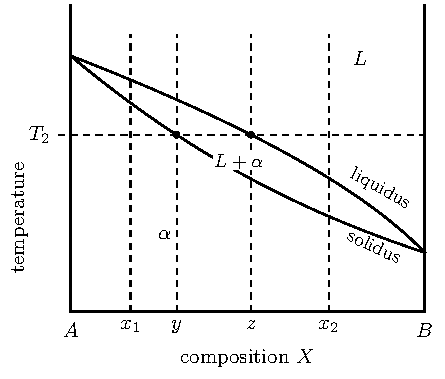
\includegraphics{figures/quiz1_lens}
\caption{Isomorphous system of Exercise~22.}
\label{fig:ex-lens}
\end{figure}
\begin{parts}
    \item Which phase is pure $B$ at $T_2$?
    \item Why can no two-phase layer form in the diffusion couple? Sketch the composition profile during diffusion.
    \item Which phases remain, and with which compositions, for the average compositions $x_1$ and $x_2$?
\end{parts}
\textit{Answer.} (a) Liquid, because $T_2$ lies above the melting point of $B$. (b) Both chemical potentials are uniform across a two-phase mixture, so no flux crosses the mixture. The profile runs from $0$ to $y$ in solid $\alpha$, jumps from $y$ to $z$ at the interface, and runs from $z$ to $1$ in the liquid. (c) For $x_1 < y$, a single solid $\alpha$ of composition $x_1$. For $x_2 > z$, a single liquid of composition $x_2$.\\
\textit{Related:} Sections~11.4, 11.8 and~11.11 of the note. \textit{Source:} Quiz~1, Problem~2.

\needspace{356pt}
\paragraph{Exercise 23: From a $P$--$T$ projection to a $T$--$X$ section.}
Figure~\ref{fig:ex-pt} shows the $P$--$T$ projection of a binary system with a eutectoid-type quadruple point $Q$.
\begin{figure}[H]
\centering
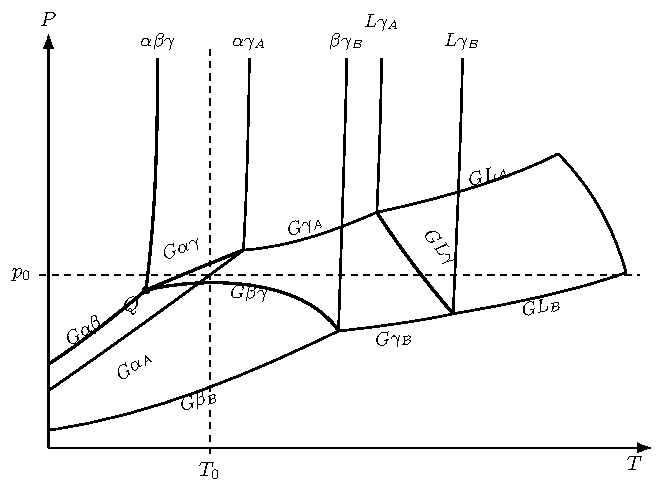
\includegraphics{figures/quiz1_pt}
\caption{$P$--$T$ projection of Exercise~23.}
\label{fig:ex-pt}
\end{figure}
\begin{parts}
    \item List the curves that the isobar $p_0$ crosses, in order of increasing temperature. Which are binary three-phase equilibria, and which belong to a pure component?
    \item For each three-phase isotherm, find the middle phase and the reaction on cooling.
    \item Draw the $T$--$X$ diagram at $p_0$.
\end{parts}
\textit{Answer.} (a) $\alpha\beta\gamma$, $G\alpha\gamma$, $G\alpha_A$, $\beta\gamma_B$, $GL\gamma$, $L\gamma_B$ and $GL_B$. The curves $\alpha\beta\gamma$, $G\alpha\gamma$ and $GL\gamma$ are binary. Pure $A$ sublimes directly at $p_0$. (b) $\gamma \to \alpha + \beta$, $G \to \alpha + \gamma$ and $L \to G + \gamma$, all of the eutectic type. (c) The two-phase regions $\alpha + G$, $\gamma + \beta$, $L + \gamma$ and $G + L$ close at the transition points of the pure components. See \texttt{quiz1.pdf}, Fig.~7.\\
\textit{Related:} Sections~11.5, 11.12 and~11.13 of the note. \textit{Source:} Quiz~1, Problem~3.

\needspace{334pt}
\paragraph{Exercise 24: Three-phase reactions in the Ag--Pr system.}
List all the three-phase reactions with liquid in Fig.~\ref{fig:ex-agpr}, with the type, the temperature and the liquid composition of each reaction.
\begin{figure}[H]
\centering
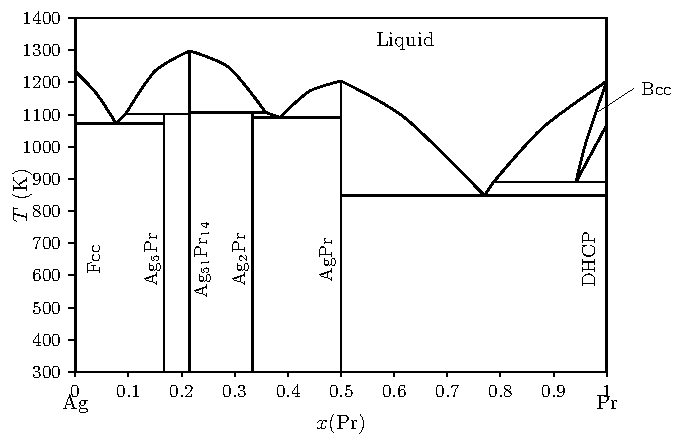
\includegraphics{figures/quiz1_agpr}
\caption{Ag--Pr phase diagram of Exercise~24.}
\label{fig:ex-agpr}
\end{figure}
\textit{Answer.} $L \to$ Fcc $+$ Ag$_5$Pr (eutectic, 1072~K, $x_L = 0.08$). $L +$ Ag$_{51}$Pr$_{14} \to$ Ag$_5$Pr (peritectic, 1102~K, $0.10$). $L +$ Ag$_{51}$Pr$_{14} \to$ Ag$_2$Pr (peritectic, 1107~K, $0.36$). $L \to$ Ag$_2$Pr $+$ AgPr (eutectic, 1091~K, $0.39$). Bcc $\to L +$ DHCP (metatectic, 890~K, $0.79$). $L \to$ AgPr $+$ DHCP (eutectic, 848~K, $0.77$). The congruent melting of Ag$_{51}$Pr$_{14}$ and AgPr involves only two phases.\\
\textit{Related:} Sections~11.5 and~11.10 of the note, Table~5. \textit{Source:} Quiz~1, Problem~4.

\needspace{359pt}
\paragraph{Exercise 25: The diopside--anorthite--albite system.}
Figure~\ref{fig:ex-tern} shows the Di--An--Ab system, with binary eutectics on the Di--An and Di--Ab sides and a solid-solution loop without a minimum on the Ab--An side.
\begin{figure}[H]
\centering
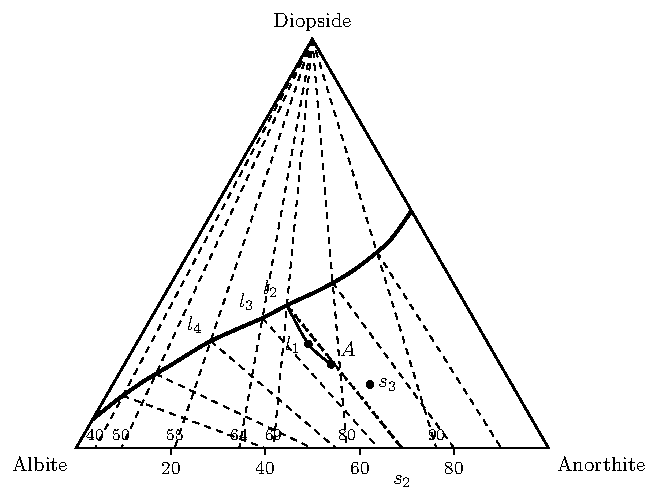
\includegraphics{figures/quiz1_ternary}
\caption{Di--An--Ab system of Exercise~25 (wt\%).}
\label{fig:ex-tern}
\end{figure}
\begin{parts}
    \item Mark the eutectic points. Why does the system have no ternary eutectic?
    \item In which directions does the temperature fall?
    \item State the meaning of the thick curve, the dashed lines from Di, the dashed lines to the Ab--An side, the curve through $l_1$ and the dotted line.
    \item Which three phases coexist along the cotectic, and which tie triangle belongs to $l_4$? Draw the isotherm through $l_4$.
    \item Read the composition of $A$, and trace the path of the liquid during equilibrium cooling of $A$. Where does crystallization end, and which plagioclase remains?
\end{parts}
\textit{Answer.} (a) $E_1$ at 58~wt\% Di on the Di--An side and $E_2$ at 7~wt\% Di on the Di--Ab side. The Ab--An loop has no minimum. (b) Along the cotectic from $E_1$ to $E_2$, along the Ab--An side from An to Ab, and in each primary field toward the cotectic. (c) Cotectic ($L$ + Di + Pl), diopside--liquid tie lines, liquid--plagioclase tie lines labeled by the An content of the plagioclase, path of the liquid, and the tie line $l_2$--$A$--$s_2$. (d) $L$ + Di + Pl. At $l_4$, the triangle Di--$l_4$--An$_{55}$. The isotherm has two branches that meet at $l_4$ in a V pointing up the cotectic. (e) $A$ = 20~wt\% Di, 44~wt\% An, 36~wt\% Ab. The path runs $A \to l_1 \to l_2$ with plagioclase alone, then along the cotectic $l_2 \to l_3 \to l_4$ with diopside and plagioclase. Crystallization ends at $l_4$ with plagioclase An$_{55}$.\\
\textit{Related:} Sections~11.4 and~11.5 of the note (ternary systems lie beyond the note). \textit{Source:} Quiz~1, Problem~5.

\end{document}
